%\documentclass{sig-alternate}
\documentclass{llncs}
\usepackage{amsmath,amssymb,graphicx}
\usepackage[ruled,linesnumbered]{algorithm2e}
\usepackage{standalone}
\usepackage{algorithmic}
\usepackage{mdwlist}
\usepackage{color}
\usepackage{multirow}
\usepackage{rotating}
\usepackage{amsmath}
\usepackage[mathscr]{eucal} %% For \mathscr
\usepackage{amsbsy} %% For \boldsymbol
\newcommand{\T}[1]{\boldsymbol{\mathscr{#1}}}  
\usepackage{booktabs}
\usepackage{tikz}
\usetikzlibrary{snakes}
\usepackage{multirow}
\usepackage{epstopdf}
\usepackage{enumitem}
\usepackage{url}
\usepackage{array}
\usepackage{pdfpages}
\setlist{nolistsep}
\newcommand{\hide}[1]{}
\usepackage{caption}
\usepackage[font={footnotesize}]{subcaption}
\captionsetup{compatibility=false}
\DeclareCaptionType{copyrightbox}
\DeclareMathOperator*{\argmin}{argmin}
\DeclareMathOperator*{\argmax}{argmax}
\newcommand{\reminder}[1]{ {\color{red} {\bf  #1} } }
\newcommand{\BigO}[1]{\ensuremath{\operatorname{O}\bigl(#1\bigr)}}

\title{Binomial and Fibonacci Heaps in Racket (rkt-heaps)}

\begin{document}

\author{
	Abhinav Jauhri\\
	\texttt{abhinavjauhri@gmail.com}\\
}

\maketitle

\begin{abstract}
	Library\footnote{A software package and will be referred as $rkt-heaps$ throughout the paper} providing data structures viz. Binomial heap \cite{vuillemin1978data} and Fibonacci heap\cite{fredman1987fibonacci} are described with primitive operations, performance and usage. 
\end{abstract}

\section{Introduction}
%\vspace{-0.1in}
$rkt-heaps$\footnote{Source code - https://github.com/ajauhri/rkt-heaps} was made for demonstration in a contest, \textit{Lisp In Summer Projects}\footnote{http://lispinsummerprojects.org/}. Any participant was expected to develop one or many applications, or libraries, using any LISP-based technology. $rkt-heaps$ uses Racket, a dialect of the Lisp language and based on the Scheme branch of the Lisp family \cite{racket_dialect}. 

\emph{Section 1 \& 2} describe Binomial and Fibonacci heaps respectively. \emph{Section 3} has performance results\footnote{Higher resolution images for all figures in this paper can be found at https://www.dropbox.com/sh/ms78nrkp0n8qh7p/G-SDznIfrc} to ascertain $rkt-heaps$ correspond to run-time bounds as shown in literature. Comparison with an existing library for Binary heaps\cite{racket_binary} in Racket is added to observe any runtime improvements in practice for operations which have similar run-time bounds in theory. \emph{Section 4} has conclusions and author's learnings. \emph{Appendix} includes syntactics of using this library in Racket. 

\section{Binomial Heaps}
Binomial heaps are a collection of heap-ordered Binomial trees with a pointer $min$ to the root of a tree having the minimum value amongst all elements in the heap. Primitive operations described in \cite{kozen1992design} are as follows: \\

\begin{enumerate}
	\item \emph{makeheap(i)} Makes a new heap with one element $i$
	\item \emph{findmin(h)} Returns the minimum value in the heap $h$
	\item \emph{insert(h, i)} Adds element $i$ to heap $h$
	\item \emph{deletemin(h)} Deletes the element with minimum value from heap $h$
	\item \emph{meld(h, h')} Combines two heaps $h$ and $h'$ into one \\
\end{enumerate}

\begin{table}
	\centering
	\begin{tabular}{| >{\centering\arraybackslash}m{1in} | >{\centering\arraybackslash}m{1in} |}
		\hline
		\centering
		Operation & Amortized Cost \\ 
		\hline
		makeheap & \BigO{1} \\[1ex]
		findmin & \BigO{1} \\ [1ex]
		insert & \BigO{1}  \\ [1ex]
		deletemin & \BigO{\log n} \\ [1ex]
		meld (eager) & \BigO{\log n}\\ [1ex]
		meld (lazy) & \BigO{1} \\ [1ex] \hline
	\end{tabular}
	\vspace{2mm}
	\caption{Amortized costs for Binomial Heaps}
	\label{tab:binomialcost}
\end{table}

Before studying costs and implementation of the above mentioned operations, explanations for certain technical terms may be helpful for the reader. 
\begin{enumerate}
	\item $Amortized\hspace{2mm} cost$ - Amortization analysis includes cost of a sequence of operations spread over the entire sequence\cite{kozen1992design}. Amortized costs may not always give the exact cost of an operation. An operation may be expensive or cheaper, but the average cost over a sequence of operations is small and defined as amortized cost.
	\item $rank$ - States the number of children of an element. For example, a Binomial tree, the tree size is $2^k$ with root at some element $e$ having rank $k$. \\
\end{enumerate} 

Making a new heap with one element - $makeheap$, and using the $min$ pointer to get the minimum value - $findmin$, both require constant number of steps. 

Insertion of a value is equivalent to making a heap, $h_1$, with a single element and then melding $h_1$ with an existing heap, $h_2$. At each step of a meld, two trees having the same rank are considered. It could be the case that either $h_1$ or $h_2$ have a tree of size $2^k$ (rank $k$), or neither have one. When two trees are combined, the resulting tree is of rank $(k+1)$. If a tree with rank $(k+1)$ already exists in either of the heaps - $h_1$ or $h_2$, then a tree of rank $(k+2)$ is made. This happens continuously till there is single tree of some rank $(>k)$ in the resulting heap, $h_{1,2}$. At the end of meld, $h_{1,2}$ has only one or no tree of size $2^i$, such that $0\le i \le \log_2 s$, where $size(h_{1,2})=s$ The heap property\footnote{Heap property ensures that all children of a tree rotted at $r$ have their values ordered with its parent's value and that the same ordering applies across the heap} is imposed each time roots of two trees are combined. For intuition on why $insert$ is \BigO{1} amortized cost consider a Binomial heap having only one tree with rank $2$. There will be no requirement to combine another tree of rank $2$ until $3$ elements have been inserted for trees with sizes $2^0$ and $2^1$. 

The technique of meld can be extended for $deletemin$ operation also; take all children of the min element and meld them with the remaining trees in the heap, and update the min pointer, costing \BigO{\log n}. For a more detailed amortized analysis, refer \cite{kozen1992design}.

$meld$ eager version works in the manner as described above but for the lazy version, all roots of one heap are added to the set of roots of the other heap. This may result in more than one binomial tree of rank $k$ in the resulting heap. Any subsequent call to a $deletemin$ operation will correct the heap such that only one binomial tree of rank $k$ exists with cost in order of \BigO{\log n}.

Binomial heap in $rkt-heaps$ is an array-based purely functional implementation leveraging Racket's $vector$ library. Purely functional ensures there are no mutations of previously created data structures. Although, this leads to anomalies in runtime costs for certain operations like \emph{insert}. With reference to Table \ref{tab:binomialcost}, the total cost for $n$ inserts is linear - \BigO{n}; but in a purely functional implementation, the insert operation cost for $n$ inserts aggregates to \BigO{n^2}. The reason for such an anomaly is due to cloning of heap vector at every insert operation. This is validated in Fig:\ref{fig:bino_anomaly}. The curve \emph{binomial-insert (quadratic)} signifies the divisor(total expected cost) for the dividend(total time) is quadratic, and hence the slope of the curve does not linearly increase with $n^2$. Since, it is amortized cost the curve will have high and low peaks instead of slope being almost zero\footnote{The ratio of the actual cost to the value expected is constant. In other words, if the cost of doing $blah$ with $foo$ data structure is \BigO{n^2}, then the ratio is $Cost_{Actual} / n^2$ should be constant}. Alternatively, taking the divisor as linear, the total run-time cost depicts a curve with slope due to increase cost of cloning the vector, which is to say that $nth$ insertion step clones the $(n-1)th$ heap vector\footnote{Racket's vector API provides \emph{(vector-append $v_1 v_2$ \dots)}, used for cloning, makes fresh copy of all elements of given vectors}. Modifying the structuring of the heap to a doubly linked list (DLL) wherein all roots of trees have pointers to its right and left root elements is imperative to ensure constant number of steps for each insert (used for analyzing run-time costs in \cite{kozen1992design}). The DLL implementation and cost shall be discussed in later sections of this paper. 

\begin{figure}
	\begin{subfigure}{0.5\textwidth}
		\centering
		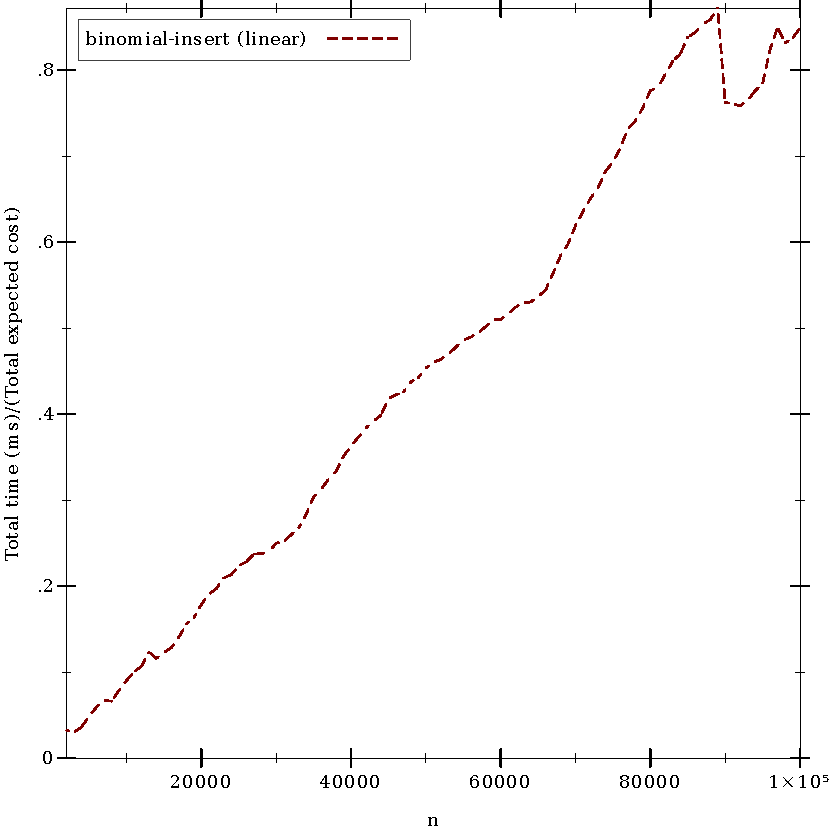
\includegraphics[width=0.8\linewidth]{FIG/insert_binomial_linear.pdf}
		\caption{Total expected cost = \BigO{n}}
		\label{fig:bino_anomaly_linear}
	\end{subfigure}%
	\begin{subfigure}{0.5\textwidth}
		\centering
		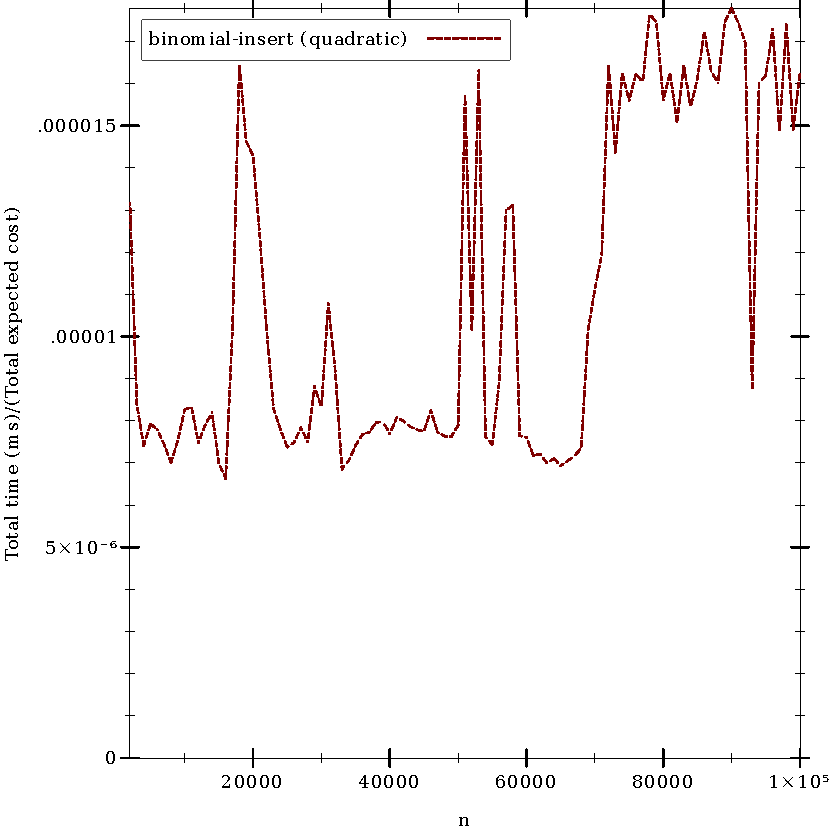
\includegraphics[width=0.8\linewidth]{FIG/insert_binomial_quad.pdf}
		\caption{Total expected cost = \BigO{n^2}}
		\label{fig:bino_anomaly_quad}
	\end{subfigure}
	\caption{Anomaly with pure functional impelementation of Binomial heaps}
	\label{fig:bino_anomaly}
\end{figure}

\section{Fibonacci Heaps}
Fibonacci heaps are a generalization of Binomial heaps. In addition to the operations provided by Binomial heaps, Fibonacci heaps provide a couple more operations. Specifically, they allow deletion of any element from the heap, and modification of value of any element provided the user has a pointer to the element. The prototypes for additional operations are as follows: \\

\begin{enumerate}
	\item \emph{decrement(h, i, $\delta$)} Decrements the value of element $i$ by $\delta$ in $h$
	\item \emph{delete(h, i)} Deletes element $i$ from the heap $h$ 
\end{enumerate}

\begin{table}
	\centering
	\begin{tabular}{| >{\centering\arraybackslash}m{1in} | >{\centering\arraybackslash}m{1in} |}
		\hline
		\centering
		Operation & Amortized Cost \\ 
		\hline
		\rule{0pt}{3ex}makeheap & \BigO{1}    \\ [1ex]
		findmin & \BigO{1} \\  [1ex]
		insert & \BigO{1}  \\  [1ex]
		deletemin & \BigO{\log n} \\ [1ex]
		meld (lazy) & \BigO{1} \\ [1ex]
		decrement & \BigO{1} \\ [1ex]
		delete & \BigO{\log n}\\ [1ex] \hline
	\end{tabular}
	\vspace{2mm}
	\caption{Amortized costs for Fibonacci Heaps}
	\label{tab:fibonaccicost}
\end{table}

Fibonacci heaps are implemented in $rkt-heaps$ using a DLL for its roots. Findings from array and functional based implementation of Binomial heaps, highlight the downsides of not having mutations which leads to much higher costs for performing primitive operations in contrast to what has been proved in literature. For this reason, Fibonacci heaps do not have a purely functional implementation in $rkt-heaps$. 

A Fibonacci heap after creation, if operated with only $deletemin$ and $meld$ operations, becomes a Binomial heap. Thus the corollary that size of tree rooted at $r$ is exponential in $rank(r)$. The exponential size of a tree is also valid when the Fibonacci heap is operated upon with $decrement$ and $delete$ operations cutting sub-tress in a controlled fashion\cite{kozen1992design}. This fact is essential to analyze amortized costs to be \BigO{1} and \BigO{\log n} for $decrement$ and $delete$ operations respectively. 

$decrement$ operation mutates the value of the element, $e$, followed by check with its parent, $p_e$, on whether the heap property is violated or not. If it is, then the sub-tree rooted at element $e$, is added to the DLL of the heap. Every parent, starting at $p_e$ is also added to DLL if a boolean flag is marked. This happens till either a root element or an element which does not have the flag marked is reached while traversing up the tree from $e$. This boolean flag is maintained for every element $e_i$, except root elements, and marked as true if one of its children have been removed or false otherwise. A sub-tree rooted at $e_i$ shall only be cut from its parent and added to DLL if a second child of $e_i$ is removed i.e. the parent element is marked and a decrement operation on a child violates the heap property or a child is deleted.

$delete$ makes the value of the element to be deleted less than the $min$ value of the heap by means of $decrement$ and then calls $deletemin$. This costs \BigO{\log n}.


\section{Evaluation}
In this section, comparisons are omitted between Binomial and Fibonacci heaps since one is purely functional and other is not. The functional technique was inefficient due to cloning of vectors as shown in Section $2$. It is trivial to build on the Fibonacci heap implementation by excluding the $decrement$ and $deletemin$ operations to get a Binomial heap with lazy melds\cite{kozen1992design} at the same cost as shown for Fibonacci heaps in this section. 

Fibonacci heap performance for operatios viz. $insert$ and $meld$ are shown in Figure \ref{fig:fi_insert_meld}. The $insert$ curve has mountainous terrain as it is the amortized total expected cost. For $meld$ the curve does not validate the fact that total expected cost should be \BigO{n}. This could be probably be due to garbage collection in Racket or some underlying implementation for creating $structures$. More work needs to be done to validate the exact cause.

\begin{figure}
	\begin{subfigure}{0.5\textwidth}
		\centering
		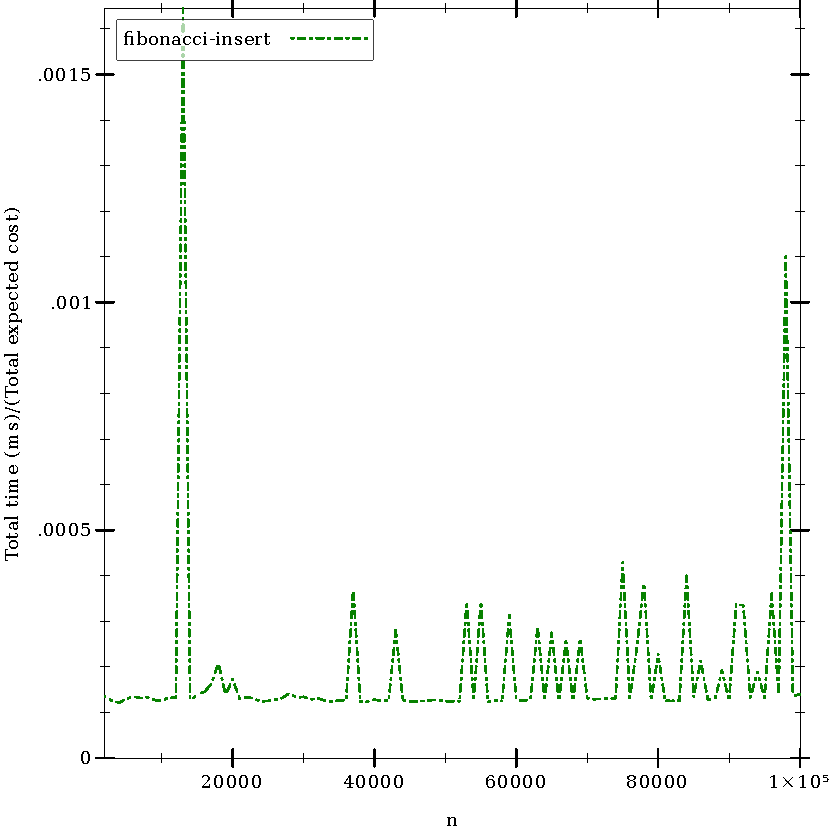
\includegraphics[width=0.8\linewidth]{FIG/fi_insert.pdf}
		\caption{Total expected cost = \BigO{n}}
		\label{fig:fi_insert}
	\end{subfigure}%
	\begin{subfigure}{0.5\textwidth}
		\centering
		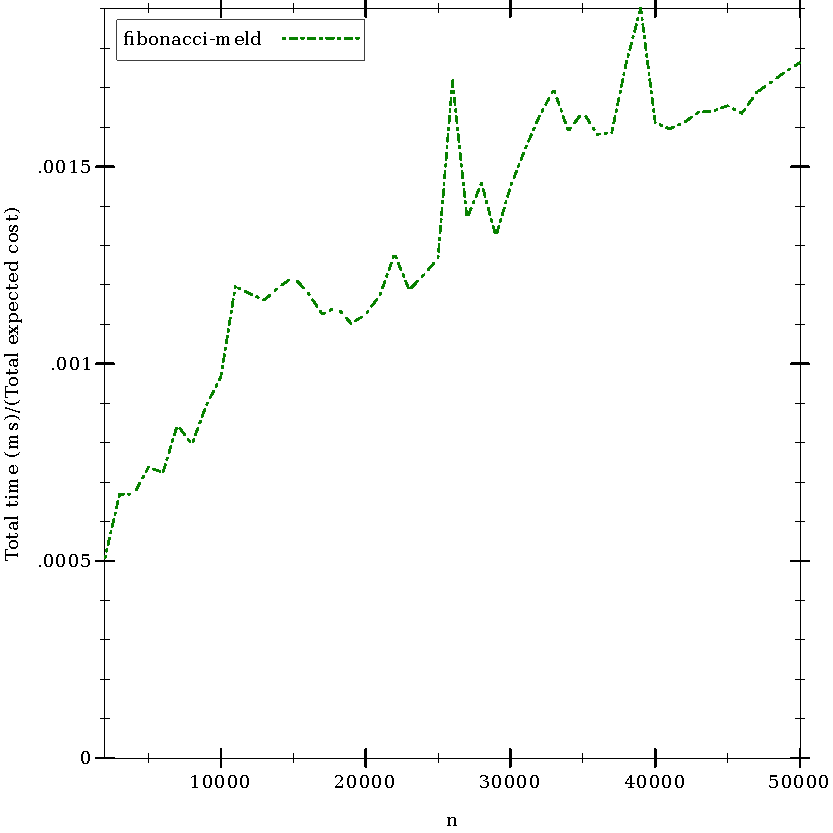
\includegraphics[width=0.8\linewidth]{FIG/fi_meld.pdf}
		\caption{Total expected cost = \BigO{n}}
		\label{fig:fi_meld}
	\end{subfigure}
	\caption{Fibonacci Heaps, $insert$ and $meld$ operations}
	\label{fig:fi_insert_meld}
\end{figure}

As stated before, $delete$ involves a call to $decrement$ to mutate the value of the node less than the $min$ value in the heap, and subsequently to $deletemin$. In Figure \ref{fig:fi_delete}, there is a very gradual increase in the slope of the curve. This is probably due to the increase in the constant, \BigO{1}, number of steps by $decrement$ operation exceeding the \BigO{\log n} number of steps by $deletemin$. It should be noted that for benchmarking a heap $h$ of size $n$, the $delete$ operation is called $n$ times, and state of $h$ is maintained in-between all $delete$ operations. To find an element to be deleted, a simple random walk is performed on $h$. Algorithm \ref{alg:rand_walk} states the random walk procedure. Therefore, for decrement operation which recursively removes parents while traversing up the graph, there is a high chance that the length of path traversed is positively correlated to number of calls to $delete$ operation $h$. As a consequence, constant cost of $decrement$ increases and thereby making the ratio of total time over total expected cost to increase with $n$ for $delete$ operation.

\begin{algorithm}[!ht]
	\caption{Random Walk for Fibonacci heap $H_f$}
	\label{alg:rand_walk}
	\begin{algorithmic}[1]
%\scriptsize
		\REQUIRE A valid fibonacci heap $H_f$ of size $S_{H_f}$
		\STATE Using the fact that the rank of $H_f \le \log_{\phi}S_{H_f}$, where $\phi$ is Golden Ratio\cite{dunlap1997golden}, uniformly select a root element, $e_{current}$
		\STATE $r:=rank(e_{current})$ 
		\STATE $d:=F_{r+2}$ where $F_i$ is the ith Fibonacci number
		\WHILE {$not\_leaf\_node(e_{current})$ and $depth(e_{current})\le d$}
		\STATE Select uniformly a child $c$, from the set of children of $e_{current}$
		\STATE $e_{current}:=c$
		\ENDWHILE
		\RETURN $e_{current}$
	\end{algorithmic}
\end{algorithm}

\begin{figure}
	\begin{subfigure}{0.5\textwidth}
		\centering
		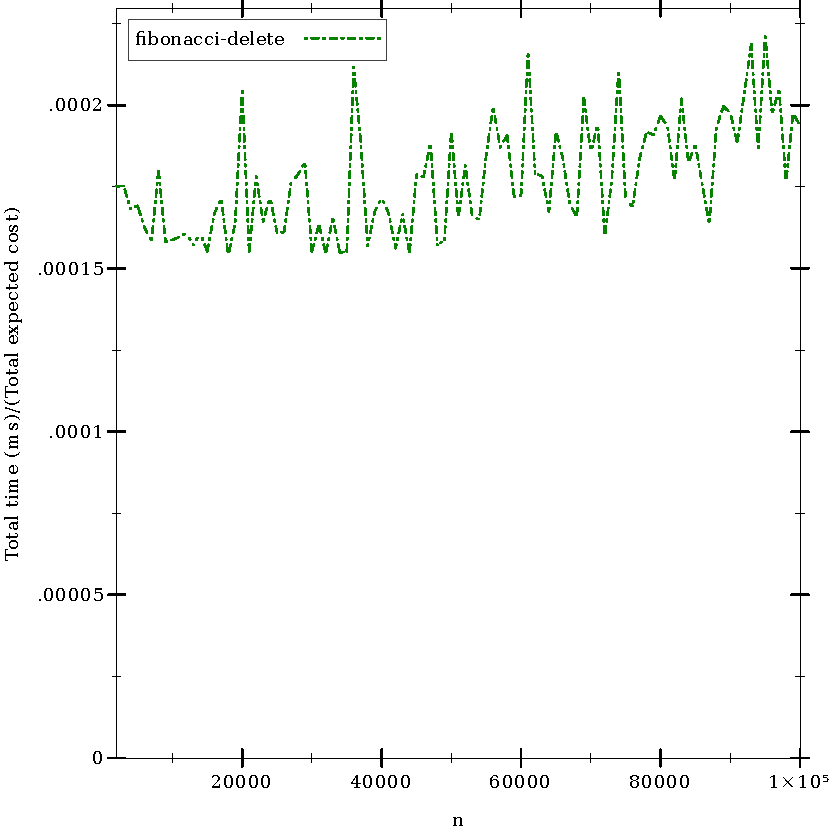
\includegraphics[width=0.8\linewidth]{FIG/fi_delete.pdf}
		\caption{Total expected cost = \BigO{n \log n}} 
		\label{fig:fi_delete}
	\end{subfigure}%
	\begin{subfigure}{0.5\textwidth}
		\centering
		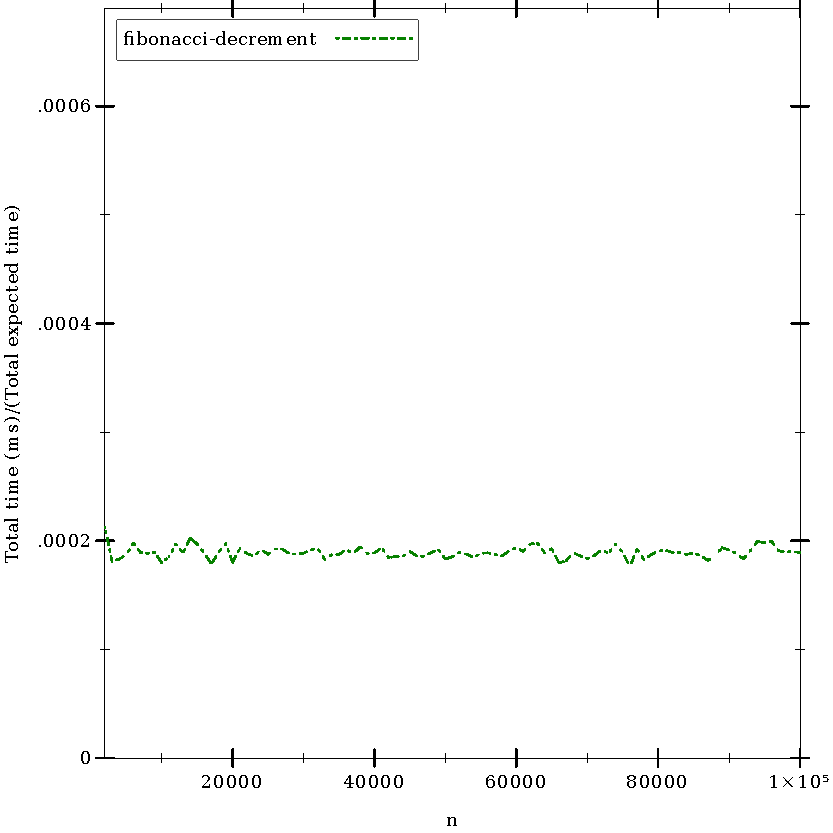
\includegraphics[width=0.8\linewidth]{FIG/fi_decrement.pdf}
		\caption{Total expected cost = \BigO{n}}
		\label{fig:fi_decrement}
	\end{subfigure}
	\caption{Fibonacci Heaps, $delete$ and $decrement$ operations.}
	\label{fig:fi_delete_decrement}
\end{figure}


Pre-packaged library for Binary heap in Racket is compared with Fibonacci implementation of $rkt-heaps$ on operations which have equal expected time bounds viz. $findmin$(Figure \ref{fig:findmin}) and $deletemin$(Figure \ref{fig:deletemin}). Fibonacci heaps outperforms Binary heaps in both operations. The equivalent operations in Binary heap library are called as $heap-min$ and $heap-remove-min$.

\begin{figure}
	\begin{subfigure}{0.5\textwidth}
		\centering
		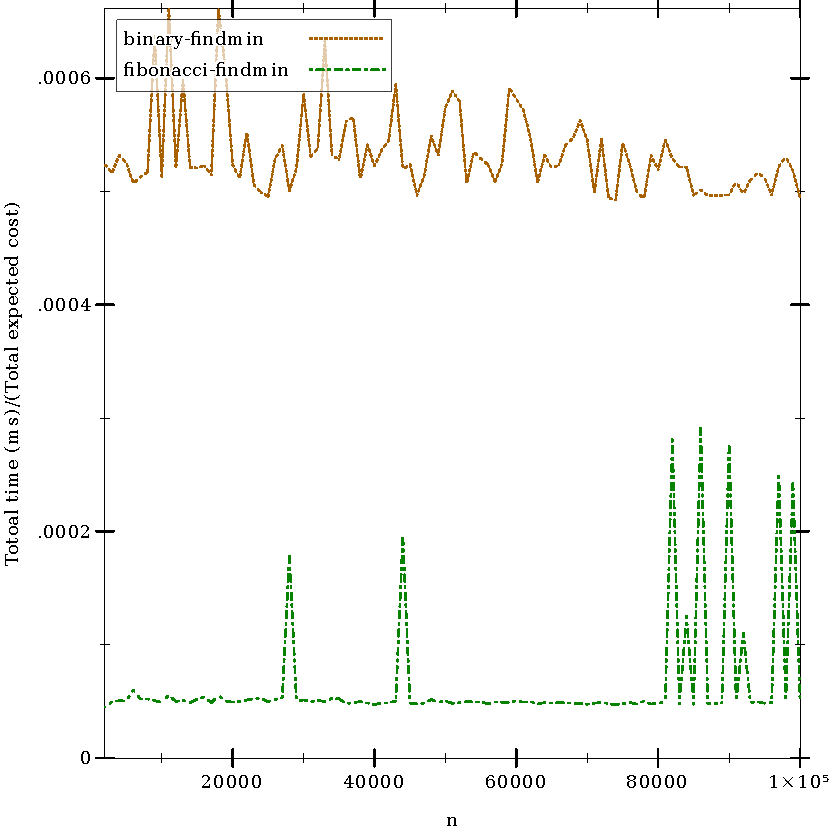
\includegraphics[width=0.8\linewidth]{FIG/findmin.pdf}
		\caption{Total expected cost = \BigO{n}}
		\label{fig:findmin}
	\end{subfigure}%
	\begin{subfigure}{0.5\textwidth}
		\centering
		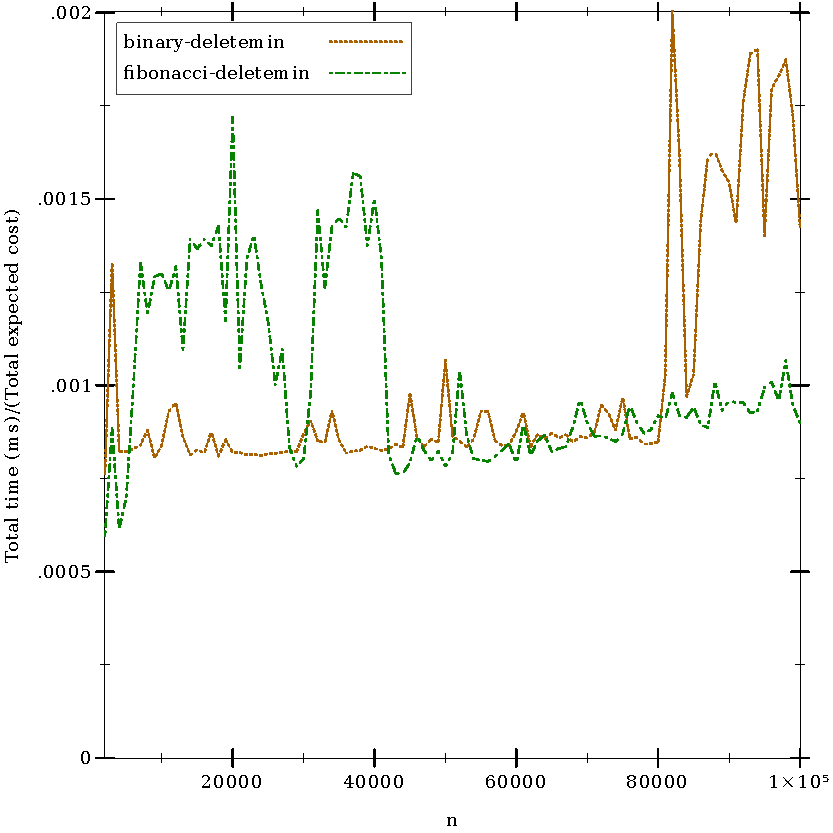
\includegraphics[width=0.8\linewidth]{FIG/deletemin.pdf}
		\caption{Total expected cost = \BigO{n \log n}}
		\label{fig:deletemin}
	\end{subfigure}
	\caption{Binary Heaps vs Fibonacci Heaps, $findmin$ and $deletemin$ operations.}
	\label{fig:fi_bi_comp}
\end{figure}

\section{Conclusions}
In this paper:
\begin{itemize}
	\item Binomial heaps included in $rkt-heaps$ do not run in expected time since they have been implemented in a functional style
	\item $rkt-heaps$ provide an efficient implementation of Fibonacci heaps using doubly linked lists (DLL)
	\item Fibonacci heaps perform better than the existing Racket library implementation of Binary heaps for comparable operations
	\item Fibonacci heaps can be easily extended to work as Binomial heaps although it will not be purely functional
\end{itemize}

\subsection{Author's learnings}
\begin{itemize}
	\item Initially, this work was started using mit-scheme but later migrated to Racket since there was better support for generation of graphs, testing and debugging
	\item Understanding functional style of implementing heaps
	\item Run-time graphs\footnote{Thanks to Dhruv Matani (http://dhruvbird.com) for his inputs in making graphs more meaningful} are essential to ascertain the algorithms were performing correctly as stated in literature
	\item Pure functional implementations can be slow 
    \item A mutation can dependent on other mutations, hence sequence of mutations is important for correctness of an operation
\end{itemize}
		

\bibliographystyle{plain}
\bibliography{BIB/refs.bib}

\newpage
\appendix
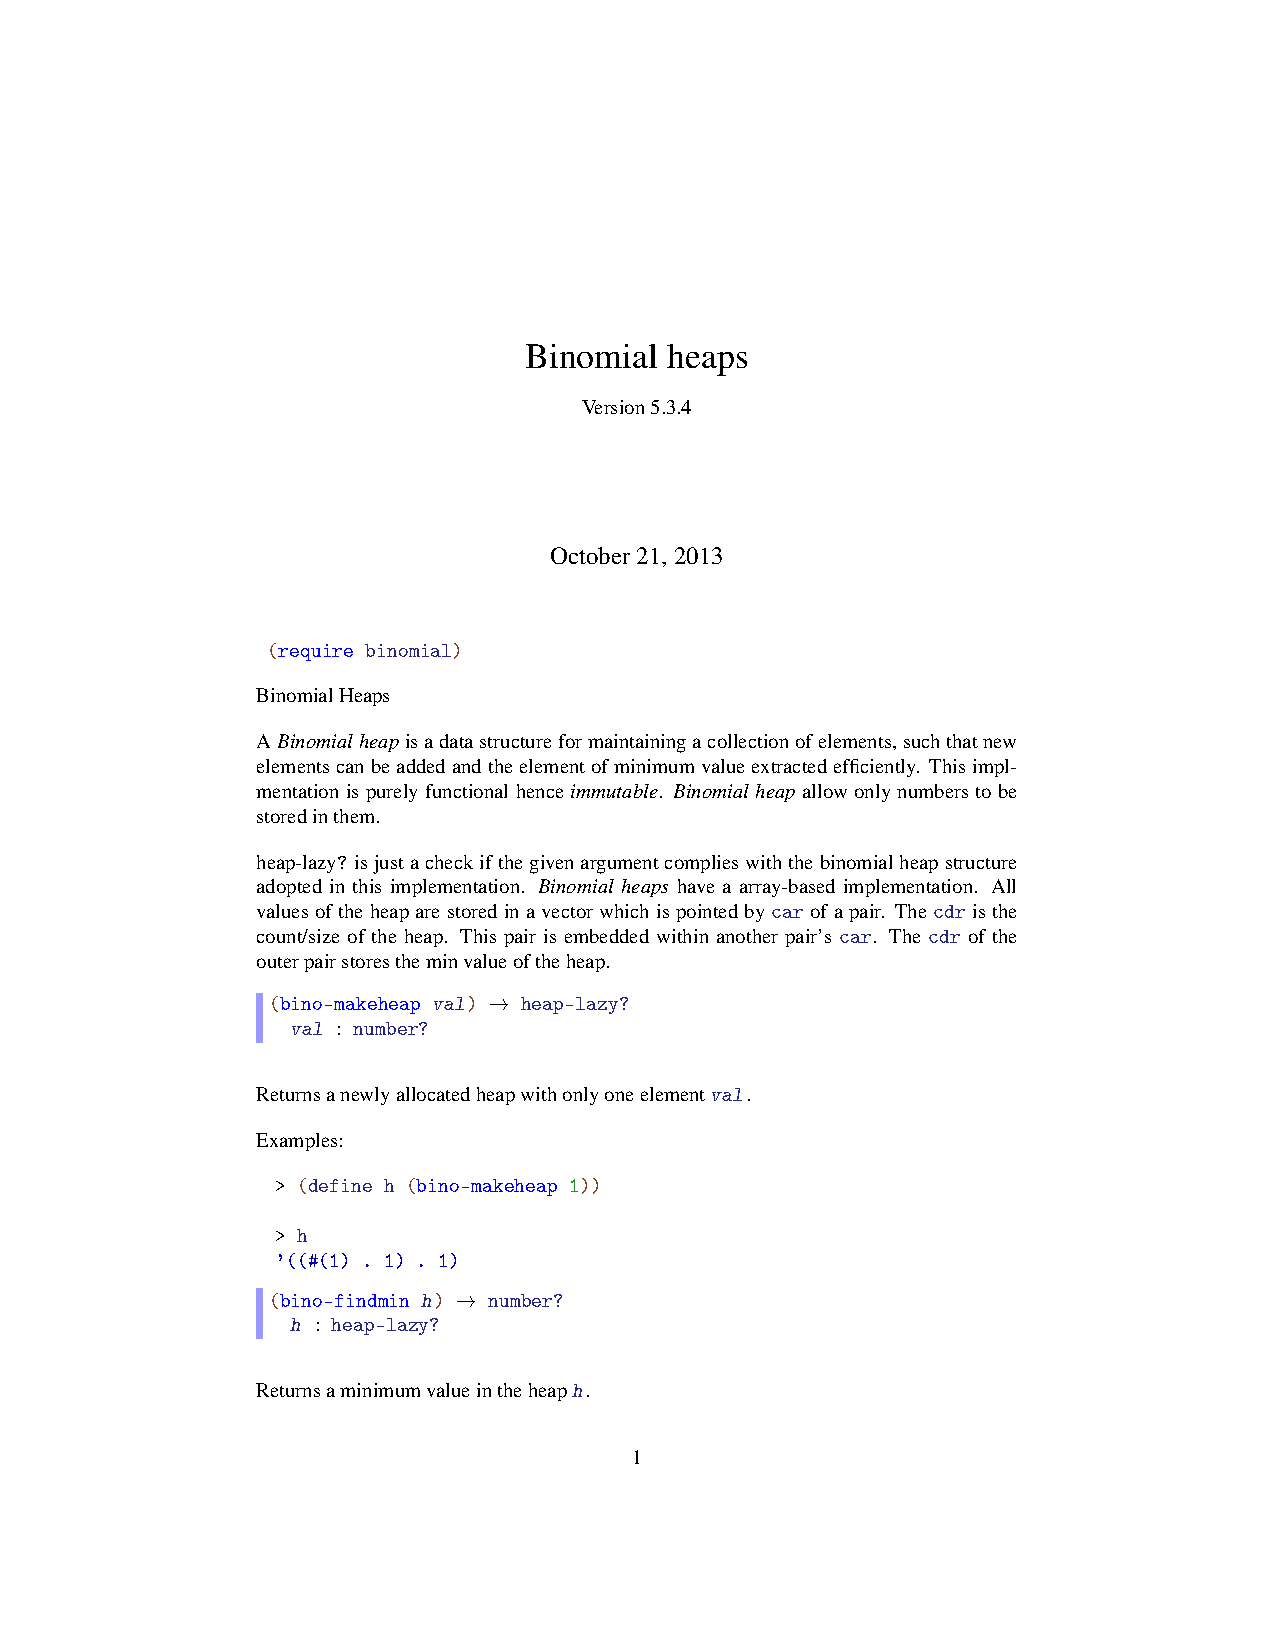
\includepdf[pages={-}]{binomial.pdf}
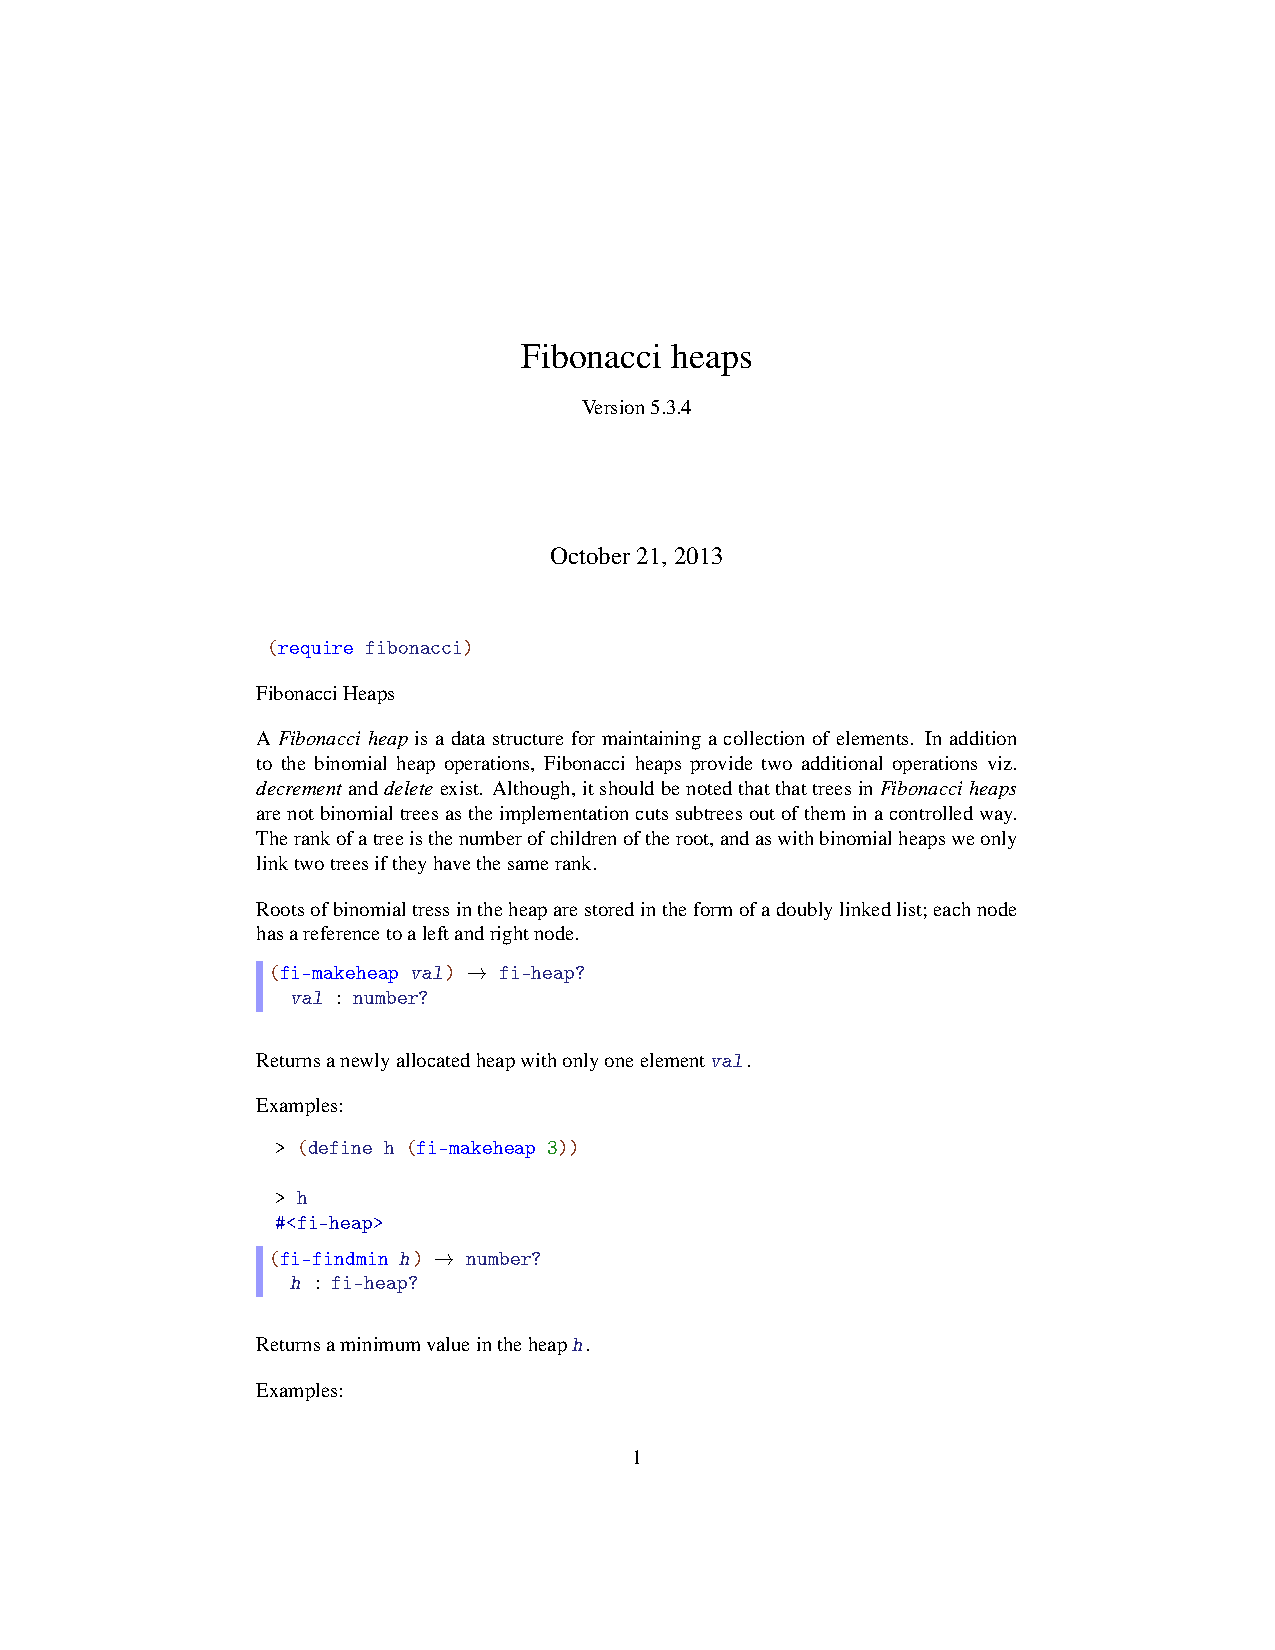
\includepdf[pages={-}]{fibonacci.pdf}
\newpage
\end{document}
